\documentclass[14pt]{beamer}
\mode<presentation>
{
\usepackage{color}
\usepackage{graphicx}
\usepackage{tikz}
\usetheme[white]{Wisconsin}
\setbeamercovered{transparent}
}

\begin{document}

\title{DAG-MCNP \& make\_watertight}
\author{Patrick C Shriwise}
\institute{University of Wisconsin - Madison}
\date{December 06, 2013}

%--- Title Frame ------------%
\maketitle


%--- Frame 2 ----------------%
\begin{frame}
\frametitle{Brief History}
\begin{itemize}
\item Undergrad at Kansas State University
\item Worked on Pegasus for 2 years at UW - Madison
\item Came to CNERG in July of 2013
\vfill
\textbf{Research goal:} \\
Improve the robustness \& performance of geometry handling in DAG-MCNP\\
(watertightness, faceting, topology)
\end{itemize}
\end{frame}

%--- Frame 3 ----------------%
\begin{frame}
\frametitle{Overview}

\begin{itemize}

\item Motivation
\item Current impact of DAG-MCNP
\item DAG-MCNP workflow
\item make\_watertight algorithm
\item Examples
\item Limitations
\item Current research

\end{itemize}
\end{frame}

%--- Frame 4 ----------------%
\begin{frame}
\frametitle{Motivation for CAD-based Monte Carlo}
\begin{itemize}
\vfill
\item Faster
	\begin{itemize}
	\item faster design iteration
	\item provides a common domain inter-analysis coupling
	\end{itemize}
\vfill
\item Cheaper
	\begin{itemize}
	\item reduced human effort
	\end{itemize}
\vfill
\item Better
	\begin{itemize}
	\item avoidance of human error
	\item ability to describe higher-order surfaces
	\end{itemize}
\end{itemize}

\end{frame}

%--- Frame 5 ----------------%
\begin{frame}
\frametitle{Impact of DAG-MCNP}
\vfill
\includegraphics[scale=0.35]{QualityGraph.png}
\end{frame}

%--- Frame 6 ----------------%
\begin{frame}
\frametitle{Impact of DAG-MCNP}
\includegraphics[scale=0.43, trim = 0 0 28 0]{InitialGraphImpact.png}
\end{frame}


%--- Frame 7 ----------------%
\begin{frame}
\frametitle{DAG-MCNP Workflow}
\includegraphics[scale=0.25, trim = 40 400 0 0]{DAGMC_Wrkflw1.png}
\end{frame}


%--- Frame 8 ----------------%
\begin{frame}
\frametitle{DAG-MCNP Workflow}
\includegraphics[scale=0.25, trim = 40 400 0 0]{DAGMC_Wrkflw2.png}
\end{frame}

%--- Frame 9 ----------------%
\begin{frame}
\frametitle{DAG-MCNP Workflow}
\includegraphics[scale=0.25, trim = 40 400 0 0 ]{DAGMC_Wrkflw3.png}
\end{frame}

%--- Frame 10 ----------------%
\begin{frame}
\frametitle{DAGMC Workflow}
\includegraphics[scale=0.25, trim = 40 400 0 0]{DAGMC_Wrkflw4.png}
\end{frame}


%--- Frame 11 ----------------%
\begin{frame}
\frametitle{DAG-MCNP Workflow}
\includegraphics[scale=0.25, trim = 40 400 0 0]{DAGMC_Wrkflw5.png}
\end{frame}

%--- Frame 12 ----------------%
\begin{frame}
\frametitle{DAG-MCNP Workflow}
\includegraphics[scale=0.25, trim = 40 400 0 0]{DAGMC_Wrkflw6.png}
\end{frame}


%--- Frame 13 ----------------%
\begin{frame}
\frametitle{DAG-MCNP Challenges}
\begin{itemize}
\vfill
\item Quality of CAD geometry
	\begin{itemize}
	\item small gaps \& overlaps
	\item lost particles
	\item previous applications of CAD analysis \\
	are less sensitive
	\end{itemize}
\vfill
\item Human efficiency gains reduced
	\begin{itemize}
	\item unique DAG-MCNP skill set required
	\end{itemize}
\vfill
\item DAG-MCNP-specific challenges
	\begin{itemize}
	\item Inconsistent faceting
	\item Robustness of tracking algorithm
	\end{itemize}
\end{itemize}
\end{frame}

%--- Frame 14 ----------------%
\begin{frame}
\frametitle{DAG-MCNP Challenges}
\begin{itemize}
\vfill

\item Quality of CAD geometry
	\begin{itemize}
	\color{red}
	\item small gaps \& overlaps
	\item lost particles
	\item previous applications of CAD analysis \\
	are less sensitive
	\end{itemize}
\vfill
\item Human efficiency gains reduce
	\begin{itemize}
	\item unique DAG-MCNP skill set required
	\end{itemize}
\vfill
\item DAG-MCNP-specific challenges
	\begin{itemize}
	\item Inconsistent faceting
	\item Robustness of tracking algorithm
	\end{itemize}
\end{itemize}
\end{frame}

%--- Frame 15 ---------------%
\begin{frame}
\frametitle{make\_watertight}
\begin{itemize}
\item Developed by Brandon Smith (2011)
\item purpose is to seal faceted CAD models using geometric information provided by CGM
\vfill
\includegraphics[scale=0.4, trim = 80 0 0 0]{sealing_ex.png}
\end{itemize}
\end{frame}

%--- Frame 16 ---------------%
\begin{frame}
\begin{itemize}
\frametitle{make\_watertight}
\item Algorithm became incompatible with external software infatstructure and has recently been revived
\item Improves the topological soundness and accuracy of geometric models
\item Recent success in applying make\_watertight to complex geometries
\end{itemize}
\end{frame}

%--- Frame 17 ---------------%
\begin{frame}
\frametitle{make\_watertight}

\begin{itemize}
\vfill
\item By definition faceted models are not watertight
	\begin{itemize}
	\item CGM faceting engine in dagmc\_preproc (same as Cubit's)
	\item surface edge vertices are not the same
	\end{itemize}
\vfill
\item sealing algorithm makes topological changes to the model for watertightness
% picture of cylinder edge

\end{itemize}
\includegraphics[scale=0.45, trim = -100 0 0 250 ]{stitch00.png}
\end{frame}


%--- Frame 18 ---------------%
\begin{frame}
\frametitle{make\_watertight}
\begin{itemize}
\item applies faceted geometric information from CGM to remove topological ambiguity from the model
\includegraphics[scale=0.4, trim = 0 0 100 150]{VolOverlap.png}
\end{itemize}
\end{frame}


%--- Frame 19 ---------------%
\begin{frame}
\frametitle{make\_watertight}
\begin{itemize}
\item Seals small gaps in volumes using faceted geometry curves
\end{itemize}
\begin{center}
\includegraphics[scale=0.25, trim = 0 200 0 0 ]{cyl_loop_close.png}
\end{center}

\end{frame}


%--- Frame 19 ---------------%
\begin{frame}
\frametitle{Recen Success}
\begin{itemize}
\item make\_watertight has (again) been able to seal complex models for analysis
\end{itemize}
\end{frame}



\end{document}


